\subsection{Near-RT state, action, and reward}
\label{subsec:ctl-state}
The near-RT controller (\texttt{ddpg\_rc\_agent.py}) builds its observation with \texttt{state\_vector()}. With two configured S-NSSAIs the dimension is $\mathrm{len}(\text{catalog})\times11+2=24$; the constructor refuses any catalog that does not contain exactly two slices. Slice order is the catalog order, so the per-slice block offset is $o=0$ for Slice~A (\snssaiA) and $o=11$ for Slice~B (\snssaiB). Table~\ref{tab:ctl-state} lists the ordered layout. The layout is pinned by unit tests in \texttt{tests/test\_services.py}, which assert the length, the individual entries, and the normalization mask.

\begin{table}[t]
\centering
\footnotesize
\caption{Ordered 24-D near-RT state. Per-slice block offset $o=0$ (Slice~A) and $o=11$ (Slice~B); indices 22--23 are global. ``RMS'' marks the six entries standardized by the running mean/variance estimator.}
\label{tab:ctl-state}
\begin{tabular}{llll}
\toprule
Index & Feature (\texttt{network\_state} source) & Range & Norm.\\
\midrule
$o{+}0$ & \texttt{dl\_th\_mbps} & Mbps & RMS\\
$o{+}1$ & \texttt{ue\_count} & count & RMS\\
$o{+}2$ & \texttt{prb\_used} share of both slices & $[0,1]$ & raw\\
$o{+}3$ & $\log(1+\texttt{dl\_buffer\_bytes})$ & nats & RMS\\
$o{+}4$ & $\texttt{wb\_cqi}/15$, $0$ if invalid & $[0,1]$ & raw\\
$o{+}5$ & \texttt{bler}, $0$ if invalid & $[0,1]$ & raw\\
$o{+}6$ & \texttt{channel\_valid} mask & $\{0,1\}$ & raw\\
$o{+}7$ & projected A1 target ratio${}/100$ & $[0,1]$ & raw\\
$o{+}8$ & last applied \texttt{dedicated\_prb}${}/100$ & $[0,1]$ & raw\\
$o{+}9$ & priority-slice one-hot & $\{0,1\}$ & raw\\
$o{+}10$ & protected-slice one-hot & $\{0,1\}$ & raw\\
\midrule
$22$ & SLA floor / calibrated capacity & $\geq0$ & raw\\
$23$ & protected-slice deficit $D_t$ & $[0,1]$ & raw\\
\bottomrule
\end{tabular}
\end{table}

Only three of the eleven per-slice features---downlink throughput, UE count, and log RLC buffer, i.e.\ state indices $\{0,1,3,11,12,14\}$---are standardized by a Welford running mean/variance estimator (\texttt{epsilon} $10^{-8}$, \texttt{clip} $5.0$, \texttt{min\_std} $0.05$). The remaining eighteen entries, including both global features, are already bounded and are passed through unchanged; \texttt{normalize\_state\_batch()} implements this as an element-wise \texttt{where} against a fixed mask. The two global features are the SLA floor divided by the calibrated cell capacity and the protected-slice deficit normalized by the floor, clipped to $[0,1]$ and forced to zero when the floor is inactive or the protected slice carries no UE. The estimator is updated only by the asynchronous learner, is frozen after \texttt{normalization\_freeze\_transitions}${}=1000$ valid transitions, and reaches the controller only inside an accepted Actor snapshot; the controller is pinned to \texttt{stats\_frozen}${}=\mathrm{True}$ from its first swap onward and never updates statistics locally. Inference-time normalization is therefore bit-identical to the learner's.

In \texttt{ddpg\_only} the state is built with \texttt{guidance\_enabled=False}, which zeroes feature $o{+}7$ for both slices. Every other entry is unchanged: the priority and protected one-hots, the calibrated floor, and the deficit all remain, because they come from the machine-readable policy context rather than from the model output. Both learning arms therefore optimize the same intent; only the LLM's proposed target, its bounds, and the teacher loss are withheld from the unguided arm. Priority and protected identities are resolved from \texttt{policy\_context.priority\_slice} and \texttt{policy\_context.protected\_slice}; regex parsing of the intent sentence is only a fallback, and in this campaign both fields are always supplied explicitly by calibration.

\paragraph*{Action projection}
The Actor emits one scalar $u=\sigma(z)\in[0,1]$. Percent bounds are converted to an integer PRB interval by \texttt{feasible\_slice\_a\_prbs()}, with ceiling on minima, floor on maxima, and an explicit complementarity constraint over the $N_{\mathrm{PRB}}=106$ cell:
\begin{align}
b_A^{\min}&=\max\!\left(\left\lceil\tfrac{r_A^{\min}N_{\mathrm{PRB}}}{100}\right\rceil,\;N_{\mathrm{PRB}}-\left\lfloor\tfrac{r_B^{\max}N_{\mathrm{PRB}}}{100}\right\rfloor\right),\\
b_A^{\max}&=\min\!\left(\left\lfloor\tfrac{r_A^{\max}N_{\mathrm{PRB}}}{100}\right\rfloor,\;N_{\mathrm{PRB}}-\left\lceil\tfrac{r_B^{\min}N_{\mathrm{PRB}}}{100}\right\rceil\right),
\end{align}
raising an error if the interval is empty. The operational envelope \texttt{control.min\_prb}${}=10$, \texttt{control.max\_prb}${}=90$ therefore yields $b_A\in[11,95]$ rather than a naive $[10.6,95.4]$. The commanded budget is $b_A=\operatorname{round}(b_A^{\min}+u(b_A^{\max}-b_A^{\min}))$ and $b_B=N_{\mathrm{PRB}}-b_A$; the emitted percentages are $r_A=\operatorname{round}(100b_A/N_{\mathrm{PRB}})$ and $r_B=100-r_A$. \texttt{policy\_from\_ratios()} writes one entry per slice with PLMN, SST, SD, \texttt{min\_prb}, \texttt{max\_prb}, and \texttt{dedicated\_prb}; \texttt{validate\_prb\_policy()} enforces $0\leq r_{\min}\leq r_{\mathrm{dedicated}}\leq r_{\max}\leq100$ and $\sum_k r_{\mathrm{dedicated},k}\leq100$; \texttt{write\_prb\_policy\_file()} writes atomically (temporary file, \texttt{fsync}, \texttt{os.replace}). For \texttt{ddpg\_only} the feasible interval is the operational envelope alone; for the guided and LLM-only arms it is the intersection of the operational envelope with the bounds carried by the active A1 policy. Exploration noise is added to $u$ before projection and clipped to $[0,1]$; its standard deviation decays linearly from $0.2$ to $0.02$ as a function of \emph{valid transitions}, not learner steps.

\paragraph*{Reward}
\texttt{reward\_components()} evaluates a two-branch reward. Let $\bar T_t$ and $\bar T^{\mathrm{pri}}_t$ be aggregate and priority-slice downlink throughput divided by the calibrated cell capacity, $U_t=\lambda_T\bar T_t+\lambda_P\bar T^{\mathrm{pri}}_t$, $D_t$ the normalized protected-slice deficit, $\overline{\mathrm{BLER}}_t$ the unweighted mean of the per-slice BLER, $C_t=\sum_k|r_{k,t}-r_{k,t-1}|/100$ the action churn, and $S_t=\max(0,\rho_{\min}-\rho^{\mathrm{pri}}_t)/100$ the shortfall of the \emph{commanded} priority ratio against $\rho_{\min}=55$. Collecting the terms that are charged in both branches into a common cost $K_t=\lambda_B\overline{\mathrm{BLER}}_t+\lambda_C C_t+\lambda_S S_t$, the implemented reward is
\begin{equation}
R_t=
\begin{cases}
U_t-K_t, & D_t=0,\\[3pt]
-\lambda_V-\lambda_D D_t-K_t, & D_t>0,
\end{cases}
\label{eq:ctl-reward}
\end{equation}
with $\lambda_T=1.0$, $\lambda_P=0.5$, $\lambda_V=1.0$, $\lambda_D=2.0$, $\lambda_B=0.2$, $\lambda_C=0.1$, and $\lambda_S=1.0$. These are the code defaults and are reproduced verbatim in the \texttt{reward} object of \texttt{config.yaml}; only keys already present in the default dictionary can be overridden. Three design points follow from~\eqref{eq:ctl-reward}. First, priority throughput earns utility only after the protected floor is met: a violated step drops the entire throughput utility and additionally incurs the fixed penalty $\lambda_V$, so the reward is discontinuous at the floor and the constrained objective of Section~\ref{subsec:objective} is enforced by construction rather than by a soft trade-off. Second, $S_t$ is the only term that couples the $55\%$ priority requirement to the reward, and it penalizes the \emph{commanded} PRB ratio rather than measured throughput, which makes the requirement directly controllable. Third, $\lambda_D$ scales a deficit that is already normalized by the floor, so the violated branch lies in $[-3,-1]$ before the common cost $K_t$ is subtracted. Churn is zero for the first action of each \texttt{run\_controller()} invocation, because the previous-ratio reference is local to that call and the v5 protocol re-enters the controller at every $60$~s training block and every intent switch.

Two satisfaction predicates are recorded and must not be conflated. \emph{SLA satisfied} means the floor is inactive or $T_{\mathrm{protected}}\geq F$. \emph{Intent satisfied} additionally requires $S_t\leq0$, i.e.\ the commanded priority slice actually received at least $\rho_{\min}=55\%$ of the PRB budget. The gap between the two drives the results discussion: a policy can hold the protected floor while persistently under-serving the priority slice.

\subsection{Control loop and transition validity}
\label{subsec:ctl-loop}
The controller runs on its own monotonic $100$~ms schedule (\texttt{period\_ms.ddpg}). On each wake it records the scheduled and actual wall-clock instants, the jitter, and $\mathrm{elapsed\_periods}=\lfloor(t_{\mathrm{now}}-t_{\mathrm{sched}})/T\rfloor+1$, then advances the next deadline by $\mathrm{elapsed\_periods}\cdot T$, so a late tick is dropped rather than accumulating drift. Every tick---including skipped ones---writes one row to \texttt{controller\_ticks} (\texttt{scheduled\_ts\_ms}, \texttt{wake\_ts\_ms}, \texttt{jitter\_ms}, \texttt{elapsed\_periods}, \texttt{state\_ts\_ms}, \texttt{state\_fresh}, \texttt{skip\_reason}, \texttt{action\_issued}, \texttt{action\_ts\_ms}, \texttt{policy\_version}). These rows are drained by a daemon \texttt{ControllerTickRecorder} thread in batches of 32, so database I/O never blocks the decision path.

Three guards skip a tick without issuing an action: \texttt{no\_state} (no \texttt{network\_state} summary), \texttt{stale\_age} (summary age above \texttt{max\_state\_age\_ms}${}=1000$), and \texttt{state\_not\_advanced} (the summary timestamp has not increased since the last action). The third guard is the design decision that matters: rather than fabricating a transition from an already-consumed observation, the controller waits for genuinely new evidence. This is why the measured fresh-state action interval exceeds the nominal $100$~ms clock.

Actions are not scored on the immediately following tick. Each issued action is appended to a pending queue holding the raw state, the commanded ratios, the training context, the governing policy version, and the actuator response timestamp. Its effect window is the half-open interval $(t_{\mathrm{ack}},\,t_{\mathrm{ack}}+\Delta]$ with $\Delta={}$\texttt{transition\_observation\_ms}${}=100$~ms. \texttt{\_effect\_window\_states()} selects every \texttt{ue\_metric\_provenance} row whose window overlaps that interval, keeps only timestamps at which \emph{both} slices have a \texttt{network\_state} row, weights each $50$~ms summary by its overlap in milliseconds, and returns a coverage fraction $\min(1,\,\text{covered}/\Delta)$. The reward is then evaluated by \texttt{\_aggregate\_reward\_states()} on the duration-weighted average of those summaries (mean of \texttt{dl\_th\_mbps}, \texttt{ul\_th\_mbps}, \texttt{prb\_used}, \texttt{bler}, \texttt{latency\_ms}; maximum of \texttt{ue\_count}), whereas the successor state $s_{t+1}$ stored in replay is the current tick's fresh $50$~ms summary. At most one pending transition is completed per tick, in FIFO order.

Actuation requires an end-to-end acknowledgement. \texttt{rc\_actuator.py} sends \texttt{\{request\_id, policy\_file\}} over the Unix socket \texttt{/tmp/llm\_hric/rc\_slice\_ctrl.sock} with a $5$~s timeout and accepts the reply only if the \texttt{request\_id} matches and \texttt{success} is true. In the C xApp, \texttt{success} is the conjunction of request parsing, policy loading, and \texttt{send\_slice\_controls()}, which in turn ANDs the \texttt{sm\_ans\_xapp\_t.success} of every \texttt{control\_sm\_xapp\_api()} call. That flag comes from \texttt{cond\_wait\_sync\_ui()} in FlexRIC's synchronous control path and is false on timeout, so an applied transition is one for which an E2 RIC CONTROL response was actually received. The reply also carries \texttt{sent\_ts\_ms} and \texttt{response\_ts\_ms}, which define the effect window above.

A transition enters replay as trainable only if \texttt{transition\_is\_trainable()} holds: the action was applied and acknowledged; at least one active UE was present; the number of validly mapped UEs equals the number of active UEs; no counter reset occurred in the window; every provenance row has \texttt{mapping\_valid} and a positive \texttt{source\_sample\_count}; and the effect coverage is at least \texttt{min\_effect\_coverage}${}=0.8$. Invalid transitions are still written and still advance the learner's cursor, but never enter the buffer. A transition is marked terminal when the governing version changes between the action and the successor state: for \texttt{ddpg\_only} this is \texttt{intent\_version}, which changes only at an intent switch, whereas for the guided arm it is the A1 policy row version, which the rApp bumps on every $10$~s publication. The guided arm therefore bootstraps over much shorter effective episodes. A terminal flag also resets the discounted-return accumulator of the reward scaler on both the controller and the learner side.

In the balanced-load seed-1 pilot the loop met its budget on all three arms. Tick wake-up jitter had a $99$th percentile of $107.02$, $66.87$, and $93.38$~ms for \texttt{llm\_guided\_ddpg}, \texttt{llm\_only}, and \texttt{ddpg\_only}; the interval between consecutive fresh-state actions averaged $103.58$, $101.26$, and $102.79$~ms with a common $95$th percentile of $166$~ms and $99$th percentiles of $231$, $208$, and $227.75$~ms. Ticks skipped for missing, stale, or unadvanced state accounted for $1.19\%$, $0.39\%$, and $1.00\%$; ticks that consumed more than one nominal period for $1.30\%$, $0.19\%$, and $0.76\%$. Apply success, mean effect coverage, and trainable-transition rate were all $1.00$, and the E2 control round trip had a $99$th-percentile latency of $2.80$, $3.10$, and $2.87$~ms. The v5 specification treats these as acceptance criteria (jitter $p_{95}\leq120$~ms and $p_{99}\leq150$~ms; fresh-state action interval $p_{95}\leq180$~ms and $p_{99}\leq300$~ms; skip rate $\leq0.5$).\ifFullCampaign\else{} These are single-run measurements and are reported as feasibility evidence only.\fi

Everything needed to reconstruct a decision offline is persisted. Each issued action writes a \texttt{ddpg\_actions} row whose \texttt{action\_json} carries the arm, the LLM action, the Actor sub-action (raw output, projected budgets, learner step count, a $0.02/0.98$ saturation flag, and the action bin), the fused action, both the effective and the operational bounds, the cell PRB count, the training context $(\ell,h,\tau,w,m)$, the full $24$-float raw state, the state-normalization statistics with their frozen flag, the phase, the serving Actor version, the swap latency, the emitted policy, and the actuator response. Each completed transition writes an \texttt{experiment\_steps} row with both raw states, the reward and all its components, the policy version, the observation-window timestamps, and the provenance record. One caveat applies to the logged \texttt{scaled\_reward} and \texttt{reward\_running\_std}: in asynchronous mode the controller's reward scaler is never updated and is not shipped in the snapshot, so those two columns are an audit copy at unit scale ($\sigma_G\approx1$ in every pilot run) and are not an applied normalization. Reward scaling happens only inside the learner, which recomputes it from the raw reward on every minibatch.

\begin{figure*}[t]
  \centering
  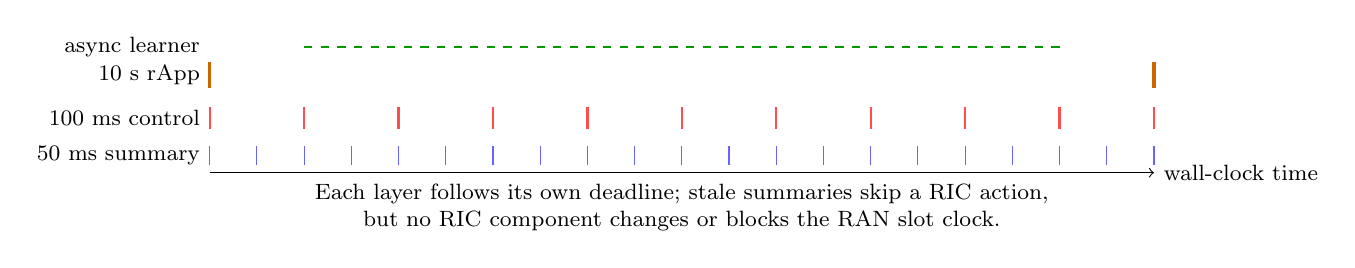
\begin{tikzpicture}[font=\footnotesize,x=0.012cm,y=0.8cm]
\draw[->] (0,0) -- (1000,0) node[right]{wall-clock time};
\foreach \x in {0,50,...,1000} \draw[blue!60] (\x,0.12)--(\x,0.42);
\node[left] at (0,0.28) {50 ms summary};
\foreach \x in {0,100,...,1000} \draw[red!70,thick] (\x,0.7)--(\x,1.05);
\node[left] at (0,0.87) {100 ms control};
\draw[orange!80!black,very thick] (0,1.35)--(0,1.75);
\draw[orange!80!black,very thick] (1000,1.35)--(1000,1.75);
\node[left] at (0,1.55) {10 s rApp};
\draw[green!60!black,thick,dashed] (100,2.0)--(900,2.0);
\node[left] at (0,2.0) {async learner};
\node[align=center] at (500,-0.55) {Each layer follows its own deadline; stale summaries skip a RIC action,\\but no RIC component changes or blocks the RAN slot clock.};
\end{tikzpicture}

  \caption{Independent clocks and data flow. RAN slot processing never waits for monitoring, LLM inference, near-RT control, or asynchronous learning.}
  \label{fig:timing}
\end{figure*}

\subsection{Guided fusion}
\label{subsec:ctl-fusion}
In \texttt{llm\_guided\_ddpg} the LLM target and the learned candidate are fused on integer PRB counts, inside the intersected bounds, rather than in normalized action space:
\begin{equation}
b_A=\mathrm{clip}\!\left(\operatorname{round}\!\left((1-w)\,b_A^{\mathrm{LLM}}+w\,b_A^{\mathrm{DDPG}}\right)+e,\;b_A^{\min},\,b_A^{\max}\right),
\label{eq:ctl-fusion}
\end{equation}
where $b_A^{\mathrm{LLM}}$ is the projected A1 target clipped to the feasible interval, $b_A^{\mathrm{DDPG}}$ is the Actor's projected budget, and $e\sim\mathcal{U}\{-2,\dots,2\}$ PRBs is a teacher-centred jitter applied only while exploring and only before $512$ valid transitions have been collected. Its purpose is to give the critic real responses around the teacher during warm-up while keeping the LLM guardrail; the commanded action, not the Actor output, is what enters replay. The learner reconstructs the continuous analogue of~\eqref{eq:ctl-fusion} as
\begin{equation}
\Pi(u;\ell,h,\tau,w)=\mathrm{clip}\!\left((1-w)\tau+w\left(\ell+u(h-\ell)\right),\,\ell,\,h\right),
\label{eq:ctl-proj}
\end{equation}
with $\ell=b_A^{\min}/N_{\mathrm{PRB}}$, $h=b_A^{\max}/N_{\mathrm{PRB}}$, and teacher $\tau=b_A^{\mathrm{LLM}}/N_{\mathrm{PRB}}$. All of $\ell$, $h$, $\tau$, $w$, and the teacher mask are persisted per transition in \texttt{ddpg\_replay\_transitions.context\_json} and \texttt{next\_context\_json}, so the learner reproduces exactly the bounds and teacher the controller saw.

The execution weight $w$ is the agent's \texttt{guided\_weight}. It starts at $0$, is explicitly reset to $0$ (together with the satisfaction history and the violation counter) after the calibration replay prefill, and is held at $0$ until $512$ valid transitions have accumulated. Thereafter \texttt{update\_guided\_safety()}---called once per completed transition with the \emph{intent}-satisfaction flag, not the SLA flag---raises it by $0.01$ at most once per ten safety updates, and only when the trailing $30$-transition history is full and at least $95\%$ satisfied. The weight is capped at \texttt{max\_ddpg\_weight}${}=0.4$, so the learned policy can never contribute more than $40\%$ of the commanded budget. On five consecutive intent violations the weight is decremented by $0.1$ and action selection forces $w=0$, reverting to the pure LLM action until satisfaction recovers. Because \texttt{update\_guided\_safety()} is invoked outside the training guard, the fusion weight and the fallback counters keep evolving during the frozen evaluation phases; only the Actor, replay ingestion, and the normalization statistics are frozen there.

Guidance also enters the loss. For guided transitions the Actor loss adds a behaviour-cloning term against the projected rApp target,
\begin{equation}
\mathcal{L}_{\mathrm{BC}}=\frac{\sum_i m_i\left(a_i^{\mathrm{proj}}-\tau_i\right)^2}{\max\!\left(\sum_i m_i,\,1\right)},\qquad a_i^{\mathrm{proj}}=\ell_i+u_i(h_i-\ell_i),
\label{eq:ctl-bc}
\end{equation}
compared in projected PRB-fraction space rather than on the raw sigmoid output. The teacher mask $m_i$ is $1$ for every non-calibration guided transition and $0$ for \texttt{ddpg\_only} and for the fixed-ratio calibration sweep. Its weight is $1.0$ for the first $500$ Actor updates and then decays linearly over $1000$ Actor updates to a floor of $0.1$, reaching that floor at Actor update $1500$. Because the guided learner performed $15{,}103$ Actor updates in the pilot, behaviour cloning operated at the $0.1$ floor for roughly $90\%$ of training.

\paragraph*{Relation to the magazine paper's three-phase schedule}
The magazine formulation of \systemname~\cite{bao2026llmhric} trains the guided agent in three discrete phases: guided exploration under the LLM teacher, policy blending with a decaying guidance weight, and self-directed operation. This deployment realizes the same progression, but as a single continuous, safety-gated schedule rather than as scheduled phase boundaries, and with the weight moving in the opposite direction. Concretely: the warm-up before $512$ valid transitions is the analogue of Phase~1---$w=0$, so the commanded action is the teacher plus a $\pm2$~PRB jitter, and the behaviour-cloning weight is at its maximum of $1.0$. The subsequent ramp is the analogue of Phase~2, except that the \emph{teacher} share $1-w$ decays instead of a guidance weight, and it decays only while measured intent satisfaction stays above $95\%$; the behaviour-cloning weight decays on its own actor-step schedule at the same time. Phase~3 is not reached in this deployment: $w$ is capped at $0.4$, so the LLM target always retains at least a $60\%$ share of the commanded budget, and a run of five intent violations returns control to the teacher entirely. The design choice is deliberate---in a live RAN the teacher is retained as a permanent safety envelope rather than as a curriculum that is eventually discarded---but it means the guided arm here is a bounded-authority controller, not the fully self-directed agent of the magazine paper's final phase. Consistently, the pilot's guided arm shows a $90.66\%$ acknowledged-action boundary rate during training, reflecting a commanded action that sits at an endpoint of a narrow calibrated interval most of the time.

\subsection{Asynchronous actor--critic learning}
\label{subsec:ctl-learner}
\paragraph*{Process split}
Inference and learning run in separate OS processes so that no gradient step can extend a control tick; Fig.~\ref{fig:async} summarizes the resulting hand-off, from replay ingestion through candidate scoring to the validated publication of a serving Actor. The campaign driver writes \texttt{effective\_config.json} into the run directory and spawns \texttt{python -m llm\_hric.ddpg\_async\_learner} with \texttt{--config}, \texttt{--run-id}, \texttt{--arm}, \texttt{--checkpoint}, \texttt{--snapshot-dir}, and \texttt{--seed}; the learner is stopped with \texttt{SIGTERM}, a $20$~s grace period, and \texttt{SIGKILL}. The controller is given one PyTorch thread and the learner two. A health check raises on the next controller tick if the learner has exited, so a dead learner fails the run rather than silently freezing the policy. In asynchronous mode the controller's own training branch is unreachable: it neither calls \texttt{train\_step()} nor updates normalization statistics nor writes checkpoints.

\paragraph*{Replay hand-off}
The two processes communicate through SQLite and one atomic file. Each completed transition is appended by \texttt{insert\_replay\_transition()} to \texttt{ddpg\_replay\_transitions}, carrying the raw state and successor state, the commanded action, the raw reward, the terminal flag, the training context and its successor, the policy version, the acknowledgement timestamp, the effect coverage, the validity flag, and the provenance record. Two indices, on \texttt{(run\_id, transition\_id)} and \texttt{(run\_id, transition\_valid, transition\_id)}, support the learner's cursor scan. Calibration-phase transitions are excluded from the controller's insert path and are instead written in bulk by the calibration prefill, which is how the buffer crosses its minimum threshold quickly. The learner polls every \texttt{learner\_poll\_ms}${}=100$~ms with a monotonic \texttt{transition\_id} cursor, reading at most \texttt{ingest\_batch\_size}${}=2048$ rows per poll; it advances the cursor over every row but admits only rows with \texttt{transition\_valid}${}=1$. Each admitted row increments a pending-update counter by one, and each poll performs $\min(32,\,\text{pending})$ gradient steps, so the update-to-data ratio is exactly one. Training is gated on \texttt{min\_replay\_transitions}${}=1000$ buffered rows; a second, lower gate inside the agent requires $128$ rows before any critic update and $512$ before any Actor update. Because publishing and training are disabled during the two frozen evaluation phases, the learner ends a run with a backlog: $15{,}519$ and $16{,}051$ untrained transitions in the guided and unguided pilot runs, against $30{,}207$ and $30{,}266$ completed updates and $45{,}726$ and $46{,}317$ valid replay rows.

\paragraph*{Algorithm}
Although the modules retain the DDPG name for continuity with the magazine paper, the learner implements a TD3-style deterministic actor--critic~\cite{fujimoto2018td3}: twin critics with a clipped double-Q target, target policy smoothing, and delayed Actor updates. The magazine deployment used plain DDPG for power allocation~\cite{bao2026llmhric}, and the code still carries that configuration as its fallback defaults---\texttt{target\_policy\_noise} $0.0$, \texttt{actor\_update\_interval} $1$, \texttt{actor\_saturation\_penalty\_weight} $0.0$, and $\gamma=0.995$. The v5 campaign configuration overrides all four ($0.1$, $2$, $0.01$, and $0.95$), and these overrides were introduced specifically to make the slicing agent converge. We attribute the need for them to the discontinuity of~\eqref{eq:ctl-reward} at the protected floor, across which a single bootstrapping critic over-estimates $Q$ and drives a bounded sigmoid action towards a rail; the clipped double-Q target, the target-action smoothing, and the saturation penalty of~\eqref{eq:ctl-actor} each counteract one part of that failure mode. Both networks are $2\times128$ ReLU MLPs with no shared trunk and no normalization layers. The Actor maps the $24$-D normalized state to a scalar through a \emph{sigmoid} output rather than a $\tanh$, because the action is a normalized PRB fraction in $[0,1]$; each critic concatenates state and action into a $25$-D input.

Per update, a batch of $128$ is drawn, rewards are rescaled as $\tilde r=\mathrm{clip}(r/\sigma_G,-10,10)$ with $\sigma_G$ the running standard deviation of the discounted return ($\gamma=0.95$), and the target is
\begin{align}
u'&=\mathrm{clip}\!\left(\pi_{\phi'}(s')+\mathrm{clip}(\epsilon,-0.25,0.25),\,0,\,1\right),\nonumber\\
a'&=\Pi(u';\ell',h',\tau',w'),\nonumber\\
y&=\tilde r+\gamma(1-d)\min_{i\in\{1,2\}}Q_{\theta_i'}(s',a'),
\label{eq:ctl-target}
\end{align}
with $\epsilon\sim\mathcal{N}(0,0.1^2)$,
$\Pi$ from~\eqref{eq:ctl-proj}, and $d$ the terminal flag. The critic loss is $\mathrm{MSE}(Q_{\theta_1}(s,a),y)+\mathrm{MSE}(Q_{\theta_2}(s,a),y)$, where $a$ is the action actually commanded on the RAN; a single Adam optimizer updates both critics. Every second step, and only once the buffer holds $512$ rows, the Actor is updated with
\begin{equation}
\mathcal{L}_{\pi}=-\mathbb{E}\!\left[Q_{\theta_1}(s,\Pi(u))\right]+\beta_t\,\mathcal{L}_{\mathrm{BC}}+\lambda_{\mathrm{sat}}\,\mathbb{E}\!\left[\left(\max(0,|z|-z_{\max})\right)^2\right],
\label{eq:ctl-actor}
\end{equation}
where $z$ are the pre-activation logits, $z_{\max}=2.944=\mathrm{logit}(0.95)$, and $\lambda_{\mathrm{sat}}=0.01$. The last term is a logit-space saturation penalty: it costs nothing while the Actor operates inside the responsive region of the sigmoid and grows quadratically once it pushes towards either rail, which prevents the gradient-starved boundary collapse that a bounded action with a discontinuous reward otherwise invites. $\beta_t$ is the behaviour-cloning weight of Section~\ref{subsec:ctl-fusion} and is identically zero for \texttt{ddpg\_only}. Gradients are clipped to norm $1.0$ separately for the joint critic parameters and the Actor. The target Actor is soft-updated only inside the delayed branch; both target critics are soft-updated every step with $\tau=0.005$. Minibatches are not drawn uniformly: \texttt{ReplayBuffer.\_balanced\_rows()} bins transitions by the commanded action into ten equal bins and round-robins over shuffled non-empty bins, which keeps the critic's action coverage broad. Per-update diagnostics (critic loss, TD error, predicted and target $Q$, Actor and behaviour-cloning losses, replay size, backlog) are persisted to \texttt{ddpg\_learner\_updates}. Table~\ref{tab:ctl-hyper} lists every hyperparameter with its configuration key. One caveat applies to reading that table against \texttt{config.yaml}: the exploration-noise decay horizon is not the only key the experiment runner rewrites at launch. Before any run starts, the runner also overrides the DDPG control period \texttt{period\_ms.ddpg} (from the spec key \texttt{control\_period\_ms}), the rApp period \texttt{period\_ms.llm} (\texttt{rapp\_period\_ms}), the monitor summary period \texttt{monitor.summary\_period\_ms} (\texttt{monitor\_summary\_period\_ms}), the operational bounds \texttt{control.min\_prb} and \texttt{control.max\_prb} (\texttt{operational\_min\_prb}, \texttt{operational\_max\_prb}), \texttt{ddpg.cell\_prbs} (\texttt{cell\_prbs}), and \texttt{ddpg.model\_version} (\texttt{ddpg\_model\_version}), each falling back to the file value when the spec omits the key. For the v5 spec the overridden values coincide with the file values, so the table is correct as printed, but \texttt{config.yaml} alone is not the record of what a run used: the runner serializes the fully merged configuration to \texttt{<run>/effective\_config.json} and passes that file to the learner, and that file is the authoritative record of the values actually in force.

\begin{table*}[t]
\centering
\footnotesize
\caption{Learner and controller hyperparameters with their \texttt{config.yaml} keys. Values are those used by the v5 campaign.}
\label{tab:ctl-hyper}
\begin{tabular}{llll}
\toprule
Config key & Value & Config key & Value\\
\midrule
\multicolumn{4}{l}{\emph{Networks and optimization} (\texttt{ddpg})}\\
\texttt{hidden\_width} & 128 & \texttt{batch\_size} & 128\\
\texttt{action\_dim} / \texttt{max\_action} & 1 / 1.0 & \texttt{replay\_size} & 100000\\
\texttt{actor\_lr} & $1\times10^{-4}$ & \texttt{gamma} & 0.95\\
\texttt{critic\_lr} (both critics) & $5\times10^{-4}$ & \texttt{tau} & 0.005\\
\texttt{gradient\_clip\_norm} & 1.0 & \texttt{action\_bins} & 10\\
\texttt{actor\_update\_interval} & 2 & \texttt{critic\_learning\_starts} & 128\\
\texttt{target\_policy\_noise} & 0.1 & \texttt{learning\_starts} & 512\\
\texttt{target\_policy\_noise\_clip} & 0.25 & \texttt{cell\_prbs} & 106\\
\texttt{actor\_saturation\_logit\_limit} & 2.944 & \texttt{actor\_saturation\_penalty\_weight} & 0.01\\
\midrule
\multicolumn{4}{l}{\emph{Exploration, normalization, transitions} (\texttt{ddpg})}\\
\texttt{exploration\_noise\_start} & 0.2 & \texttt{exploration\_noise\_end} & 0.02\\
\texttt{exploration\_noise\_decay\_steps} & 14400 (spec-derived) & \texttt{normalization\_freeze\_transitions} & 1000\\
\texttt{state\_normalization} & $\epsilon\,10^{-8}$, clip 5.0, min std 0.05 & \texttt{reward\_scaling} & $\gamma$ 0.95, clip 10.0\\
\texttt{max\_state\_age\_ms} & 1000 & \texttt{transition\_observation\_ms} & 100\\
\texttt{min\_effect\_coverage} & 0.8 & \texttt{checkpoint\_interval\_transitions} & 250\\
\midrule
\multicolumn{4}{l}{\emph{Guidance and safety} (\texttt{ddpg})}\\
\texttt{max\_ddpg\_weight} & 0.4 & \texttt{guided\_weight\_update\_interval} & 10\\
\texttt{sla\_window} & 30 & \texttt{sla\_fallback\_windows} & 5\\
\texttt{bc\_full\_weight\_actor\_steps} & 500 & \texttt{bc\_decay\_actor\_steps} & 1000\\
\texttt{min\_bc\_weight} & 0.1 & & \\
\midrule
\multicolumn{4}{l}{\emph{Asynchronous learning} (\texttt{ddpg.async\_training})}\\
\texttt{learner\_poll\_ms} & 100 & \texttt{ingest\_batch\_size} & 2048\\
\texttt{max\_catchup\_updates} & 32 & \texttt{min\_replay\_transitions} & 1000\\
\texttt{publish\_every\_actor\_updates} & 50 & \texttt{publish\_min\_interval\_s} & 5\\
\texttt{promotion\_holdout\_size} & 1024 & \texttt{snapshot\_poll\_ms} & 500\\
\texttt{max\_promotion\_saturation} & 0.4 & \texttt{max\_promotion\_q\_drop} & 0.02\\
\texttt{max\_promotion\_action\_shift} & 0.2 & \texttt{force\_promotion\_after\_rejections} & 6\\
\texttt{checkpoint\_every\_updates} & 250 & \texttt{require\_initial\_snapshot} & true\\
\texttt{initial\_snapshot\_timeout\_s} & 120 & \texttt{controller\_torch\_num\_threads} & 1\\
\bottomrule
\end{tabular}
\end{table*}

\paragraph*{Candidate promotion}
The learner does not push weights to the controller directly. A candidate is proposed only when at least $50$ Actor updates and $5$~s have elapsed since the last proposal. The candidate is the \emph{target} Actor, and it is scored against the learner's local copy of the currently serving Actor on the most recent $\min(1024,|\mathcal{B}|)$ replay rows, replaying each row's recorded $\ell,h,\tau,w$. Six gates are evaluated in order and each carries a fixed rejection string: (i) all target-Actor parameters and all candidate outputs must be finite; (ii) the saturation rate, the fraction of candidate outputs at or beyond $0.05$ and $0.95$, must not exceed $0.40$; (iii) the mean $Q$ of the candidate's executed action, computed with critic~1 only, must not fall more than $0.02$ below the serving Actor's; (iv) the mean absolute shift of the executed action versus the serving Actor must not exceed $0.20$; (v) the raw outputs must satisfy $0\leq u_{\min}\leq u_{\max}\leq1$; and (vi) the projected action must lie inside $[\ell-10^{-6},h+10^{-6}]\cap[0,1]$ for \emph{every} holdout row. Note that this promotion saturation threshold ($0.05/0.95$, applied to the target Actor on the holdout) is a different quantity from the Actor saturation rate reported in the results, which \texttt{analyze\_results.py} defines as the fraction of raw serving-Actor outputs at or beyond $0.02$ and $0.98$; the two must not be equated.

Because a drifting critic can reject every candidate and starve the controller on a stale or near-random serving Actor---the motivation stated in the source---a fallback force-promotes a candidate after \texttt{force\_promotion\_after\_rejections}${}=6$ consecutive rejections. The forced path still requires gates (i), (v), and (vi); only the saturation, $Q$-drop, and action-shift margins are waived. The rejection counter resets on any acceptance, so the serving Actor can be at most five consecutive candidate evaluations stale. Every candidate, accepted or not, is recorded in \texttt{ddpg\_actor\_versions} with its reason string and full metrics blob, and the version counter increments on every candidate, so version numbers index candidates rather than served snapshots. In the pilot the guided run accepted $62$ of $257$ candidates and the unguided run accepted all $257$; the per-candidate use of the forced path is recorded in the artifact's \texttt{ddpg\_actor\_versions.reason} and \texttt{metrics\_json.forced} fields and is provably zero for the unguided run, which had no rejections.

\paragraph*{Snapshot transport and swap}
An accepted candidate is serialized to \texttt{actor-v\{version\}.pt} via a temporary file and \texttt{os.replace}, its SHA-256 digest is computed by streaming the file, and a manifest \texttt{serving\_actor.json} is written the same way, so the payload always lands before the manifest that references it. The payload carries the target Actor weights, the state normalization statistics, the model and state-feature versions, the state and action dimensions, and a configuration fingerprint---itself a SHA-256 over the slice catalog, feature and model versions, hidden width, action dimension, and cell PRB count. A daemon watcher thread in the controller polls the manifest every $500$~ms, requires a strictly newer version and a matching run identifier, recomputes and compares the digest, loads the payload, and requires the fingerprint to match before staging a deep-copied standby Actor and standby statistics; any torn, foreign, or mismatched snapshot is silently ignored. Only the newest validated snapshot is retained, so intermediates may be skipped. The swap itself is the first thing a controller tick does after schedule bookkeeping and the health check, before state is fetched, and is pure pointer assignment. It was measured at a worst case of $0.662$~ms (guided) and $0.538$~ms (unguided) in the pilot. Before training starts, \texttt{require\_initial\_snapshot} forces the controller to block until a validated Actor and its statistics have been swapped in, with a $120$~s deadline; before each evaluation phase the watcher performs one last swap and is then frozen, which the data confirms with exactly one serving version observed in each evaluation phase for all three arms. Two caveats apply when quoting swap counts: the watcher retains only the newest pending snapshot, and the swap-latency variable is local to a \texttt{run\_controller()} call and is discarded at each block boundary. The number of distinct serving versions actually observed in \texttt{ddpg\_actions} ($61$ guided, $244$ unguided) is therefore the correct measure, not the recorded swap-latency count ($50$ and $204$).

\begin{figure}[t]
  \centering
  \begin{tikzpicture}[font=\scriptsize,node distance=5mm,
 box/.style={draw,rounded corners=2pt,align=center,minimum width=.72\columnwidth,minimum height=7mm},
 arrow/.style={-{Latex[length=1.7mm]},thick}]
\node[box,fill=blue!8] (replay) {Raw replay: $s_t$, ACK action, $r_t$, $s_{t+1}$, provenance};
\node[box,fill=green!10,below=of replay] (learn) {Independent learner: twin critics, delayed Actor update};
\node[box,fill=orange!10,below=of learn] (validate) {Holdout validation: finite, legal, Q, shift, saturation};
\node[box,fill=red!6,below=of validate] (serve) {Atomic serving-Actor swap at controller tick};
\draw[arrow] (replay)--(learn);
\draw[arrow] (learn)--(validate);
\draw[arrow] (validate)--(serve);
\end{tikzpicture}

  \caption{Asynchronous learner and validated serving-Actor publication.}
  \label{fig:async}
\end{figure}

\subsection{Trained-agent reuse}
\label{subsec:ctl-reuse}
Every learning run archives its agent as \texttt{ddpg.pt} in the run directory. The checkpoint holds the Actor, both critics, all three target networks, both Adam optimizer states, the state normalization and reward scaler states, the replay buffer, the learner counters (\texttt{train\_steps}, \texttt{actor\_update\_steps}, \texttt{valid\_transitions}, \texttt{last\_replay\_transition\_id}, \texttt{actor\_version}), the guided-safety state (\texttt{guided\_weight}, \texttt{sla\_history}, \texttt{consecutive\_violations}, \texttt{safety\_update\_steps}), the seed, and both the Python and PyTorch RNG states. Loading hard-fails on any mismatch of \texttt{model\_version}${}=4$, \texttt{state\_feature\_version}${}=3$, \texttt{replay\_schema\_version}${}=3$, state dimension, or action dimension, so an incompatible agent can never be silently reused. The learner writes a slim checkpoint (replay omitted, because serializing it dominates file size at hundreds of megabytes) every $250$ training steps and one full checkpoint on shutdown.

Two re-evaluation paths are provided, and neither modifies the source checkpoint. The first is offline and needs no RAN stack:
\begin{quote}\footnotesize\ttfamily
python -m llm\_hric.experiments.eval\_checkpoint\\
\ \ --checkpoint <run>/ddpg.pt\\
\ \ --db <run>/llm\_hric.sqlite3\\
\ \ --phase training --limit 20000\\
\ \ --plot <run>/policy\_response.png
\end{quote}
It reads the most recent valid rows of \texttt{ddpg\_replay\_transitions}, runs the deterministic Actor without exploration noise, applies~\eqref{eq:ctl-proj} with each row's recorded $\ell,h,\tau,w$, and reports the loaded counters, the mean and $95$th-percentile disagreement in PRBs between the deterministic policy and the actions that were executed live, the Actor saturation rate, and---split by intent direction using the Slice-A priority one-hot at state index $9$---the allocation mean, standard deviation and range, the mean critic $Q$, and the mean recorded reward. The optional plot writes a per-intent allocation histogram with reference lines at $45\%$ and $55\%$.

The second re-runs the full protocol against a frozen policy on the live testbed, taking roughly twelve minutes per run:
\begin{quote}\footnotesize\ttfamily
python -u -m llm\_hric.experiments.experiment\_runner\\
\ \ --spec llm\_hric/experiments/five\_ue\_traffic\_scenarios\_v5.json\\
\ \ --results /tmp/llm\_hric/experiments/five-ue-traffic-v5-eval\\
\ \ --manage-stack --seed 1 --fail-fast\\
\ \ --scenario balanced --arm ddpg\_only\\
\ \ --eval-checkpoint <run>/ddpg.pt
\end{quote}
This mode requires \texttt{--arm} and an existing file, copies the checkpoint into a fresh run directory, disables asynchronous training so that no learner is spawned and the controller takes the synchronous path with training and exploration off, and raises if the checkpoint fails to load. It skips calibration-guidance collection, the calibration replay prefill, and the entire training phase, validating only the calibration and the two evaluation phases. The run identifier carries an \texttt{-evalck} tag, the manifest records \texttt{"mode": "eval\_checkpoint"} together with the source path, and such runs are excluded from resume bookkeeping so that they can never mask a real training run. Results are scored with the same \texttt{analyze\_results.py} pipeline pointed at the dedicated results directory. Both paths, the checkpoint format, and the campaign specification are part of the released artifact at \codeurlprinted.

\begin{table*}[t]
\centering
\caption{Application interfaces, inputs, outputs, and clocks.}
\label{tab:apps}
\begin{tabular}{lllll}
\toprule
Component & Input & Output & Interface/store & Nominal period\\
\midrule
SM monitor & MAC/RLC/PDCP/GTP indications & raw counters, slice summaries & E42, SQLite & 10~ms / 50~ms\\
KPM collector & E2SM-KPM indications & audit measurements & E2, SQLite & configured subscription\\
Gemma rApp & intent, three 10~s windows & target, bounds, confidence & A1-like HTTP/SQLite & 10~s\\
near-RT controller & 24-D state, active policy & complementary PRB budgets & Unix socket, E2SM-RC & 100~ms\\
asynchronous learner & valid replay rows & validated Actor snapshot & SQLite table, atomic file & 100~ms poll\\
serving-Actor watcher & snapshot manifest & staged Actor + statistics & sha256-verified file & 500~ms poll\\
OAI scheduler & active dedicated ratios & per-slot new-data grants & gNB internal & slot-level\\
\bottomrule
\end{tabular}
\end{table*}
